\chapter{Performance}
\label{ch:p1:performance}

To obtain preliminary indications of the performance of the QUDA library on GPUs on the typical problem sizes and parameters relevant to our physics programme, we compare two kernels, namely the application of the Dirac operator in double precision and the inversion of the Dirac operator, with their native implementations on CPU in openQxD.
Seeing as the performance of the application of the Dirac operator depends only on the problem size and the boundary conditions, and not other physics parameters, we can easily test it on synthetic data for various configurations including full weak-scaling tests.
On the other hand, the convergence of iterative solvers depends on the condition of the Dirac operator and therefore the gauge field configuration, and in this case we use representative background gauge field configurations and parameters from the Markov chain ensembles which are described in \cref{tab:ensembles}.
For the comparison of the inversions between CPU and GPU implementations, we note that the multi-grid algorithm implemented in QUDA is not exactly the inexact deflation available in openQxD, therefore we anticipate further optimization of its parameters will improve its performance in future.

\begin{table}[h]
\centering
\begin{tabular}{ccccc}
Name & Global size $V_\mathrm{G}$ & Pion mass & Boundary conditions \\
\hline
G8   & $64^3 \times 128$ & $180$ MeV & periodic \\
C380 & $48^3 \times 96$  & $380$ MeV & C$^\star$ \\
\end{tabular}
\caption{The lattice ensembles used for the performance tests of the inversion of the Dirac operator. G8 has been generated by the CLS initiative~\cite{online:cls}, while C380 is generated by the RC$^\star$ collaboration~\cite{RCstar22}. The last column refers to spatial boundary conditions.}
\label{tab:ensembles}
\end{table}

\subsection{Hardware specifications}
\label{sec:hardware}

The performance measures that follow are obtained on the machines
\begin{itemize}
    \item Piz Daint multicore at CSCS, Switzerland, 2x Intel® Xeon® E5-2695 v4 @ 2.10GHz (2x 18 cores, 64/128 GB RAM)
    \item Piz Daint hybrid at CSCS, Switzerland, 1x Intel® Xeon® E5-2690 v3 @ 2.60GHz (12 cores, 64GB RAM) and 1x NVIDIA® Tesla® P100 16GB
    \item LUMI-C at CSC, Finland, 2x AMD EPYC 7763 @2.45GHz (2x 64 cores, 256-1024 GB RAM)
    \item LUMI-G at CSC, Finland, 1x AMD® Trento™ (64 cores, 512 GB RAM) and 4x AMD® Instinct™ MI250X GPU 128GB
\end{itemize}

\subsection{Dirac operator}

We investigate the scaling behaviour of applying the Dirac stencil operator, \cref{eq:Dw,eq:Dw2}, both in openQxD as well as  QUDA, see \cref{fig:daint_dw_strong,fig:daint_dw_weak,fig:lumi_dw_strong,fig:lumi_dw_weak}. We see very good strong and weak scaling on the CPU. Notice that the base case of the GPU version is one GPU (i.e. no network communication) for the periodic lattice and 8 GPUs for the C$^\star$ lattice \footnote{The current implementation demands a process grid length of at least 2 in every direction that is a spatial C$^\star$-direction. With 3 C$^\star$ directions this gives a minimum of 8 processes, i.e. 8 GPUs unless one uses MPS or MIG.}. We use 32 and 128 ranks per node in the CPU runs for Piz Daint and LUMI-C, respectively. The GPU runs are limited by network communication more severely than the CPU runs. For the weak scaling plots we make sure that node- and GPU-local lattices have the same size. The strong and weak scaling seems less favourable on the GPU, but when comparing the time to solution, we see a $\sim10$x speedup between CPU and GPU runs for the same problem size and moderate amounts of GPUs. In \cref{fig:daint_dw_weak} right, we observe the (expected) $\sim2$x slowdown of a C$^\star$ operator compared to a periodic one on the same device and setup, due to a doubling of the lattice size in $x$-direction.

The poor scaling of the application of the Dirac operator on LUMI-G (\cref{fig:lumi_dw_strong,fig:lumi_dw_weak}) can probably be explained by the high computational performance of the MI250 which exposes us to the limited communication bandwidth earlier. To make best use of resources a larger local volume would be favourable to keep the device utilized while reducing the communication overhead (due to a smaller surface-to-volume ratio). In our tests, we use the same lattice size on Piz Daint as well as on LUMI-G to be able to compare them, and the P100 with 16GB DRAM on Piz Daint was the limiting factor. However, this suggests that the way we've implemented C$^\star$ boundaries (namely by doubling the lattice) is favourable for the GPU, because it makes the local lattice larger.

\begin{table*}
\begin{tabular}{l|ll|ll}
\toprule
 & \multicolumn{4}{c}{cost in node-seconds [sec]} \\
\midrule
 & \multicolumn{2}{c}{periodic ($V_\mathrm{G}=64\times32\times32\times64$)} & \multicolumn{2}{c}{C$^\star$ ($V_\mathrm{G}=128\times64\times64\times64$)} \\
\midrule
nodes/GPUs & Piz Daint GPU & Piz Daint CPU & Piz Daint GPU & Piz Daint CPU \\
\midrule
   1 & 0.023146040(628) &  0.162241(174) &              &  1.2444(117) \\
   2 &    0.023661(178) &  0.163499(376) &              & 1.24068(475) \\
   4 &    0.025835(708) &   0.17126(101) &              & 1.32666(613) \\
   8 &    0.042252(302) &  0.174588(889) & 0.23470(762) &  1.3596(146) \\
  16 &     0.06203(113) &   0.18817(131) & 0.31696(994) & 1.44997(168) \\
  32 &     0.07759(142) &   0.18814(254) & 0.40192(427) &  1.5171(143) \\
  64 &     0.09055(397) &   0.20222(196) & 0.47902(636) &  1.5349(228) \\
 128 &    0.111636(701) &   0.26917(683) & 0.58217(911) &  1.6314(153) \\
 256 &     0.22056(302) &   0.34688(534) &  0.6954(230) &  1.8859(191) \\
 512 &     0.35585(533) & 0.434372608(0) &  0.9402(558) &  2.0787(331) \\
1024 &       0.667(141) &                &  1.2964(951) &              \\
\bottomrule
\end{tabular}
\caption{Cost in node-seconds of one application of the Dirac operator on Piz Daint (see \cref{sec:hardware}). The global lattices are held constant.}
\label{tab:nodehours_daint}
\end{table*}

\begin{table*}
\begin{tabular}{ll|ll|ll}
\toprule
 && \multicolumn{4}{c}{cost in node-seconds [sec]} \\
\midrule
 && \multicolumn{2}{c}{periodic ($V_\mathrm{G}=64\times32\times32\times64$)} & \multicolumn{2}{c}{C$^\star$ ($V_\mathrm{G}=128\times64\times64\times64)$} \\
\midrule
nodes & GPUs & LUMI GPU & LUMI CPU & LUMI GPU & LUMI CPU \\
\midrule
  1 &    1 & 0.015923220(595) &               &              &              \\
  1 &    2 &   0.0077102(141) &               &              &              \\
  1 &    4 &    0.005683(714) &               &              &              \\
  1 &    8 &    0.005751(579) & 0.044532(772) & 0.03834(325) & 0.34713(141) \\
  2 &   16 &    0.008744(472) & 0.045384(362) & 0.04359(476) & 0.35914(313) \\
  4 &   32 &     0.01111(239) &  0.04758(468) &  0.0635(125) & 0.37067(156) \\
  8 &   64 &     0.01123(100) & 0.047173(458) &  0.0724(160) & 0.40354(185) \\
 16 &  128 &     0.01679(148) &  0.04909(394) &  0.0726(118) & 0.40973(421) \\
 32 &  256 &     0.02214(183) & 0.047487(869) &  0.0926(169) & 0.40900(786) \\
 64 &  512 &     0.03478(155) & 0.052639(898) &  0.1212(206) &   0.538(118) \\
128 & 1024 &     0.05901(380) &  0.06068(222) &  0.1654(113) &              \\
\bottomrule
\end{tabular}
\caption{Cost in node-seconds of one application of the Dirac operator on LUMI-G and LUMI-C (see \cref{sec:hardware}).  The global lattices are held constant. Notice that we count $8$ GPUs per node on LUMI-G, since one AMD MI250 abstracts itself as $2$ GPUs from the point of view of the program.}
\label{tab:nodehours_lumi}
\end{table*}

In conclusion, we see a speedup for the time to solution, even if the strong and weak scaling seem poor for the GPU runs. However, we expect better scaling for larger problem sizes with a small surface to volume ratio.

Finally, looking at the cost in terms of node-hours, \cref{tab:nodehours_daint,tab:nodehours_lumi}, we see that the GPU runs are cheaper by nearly an order of magnitude. LUMI-G is a clear winner here. % that's the only case where lumi wins ...
When comparing the cost of periodic and C$^\star$, notice that the physical lattice for the C$^\star$ runs is $4$x larger than the periodic one: a factor of $4$ is thus expected.

\begin{figure}
    \centering
    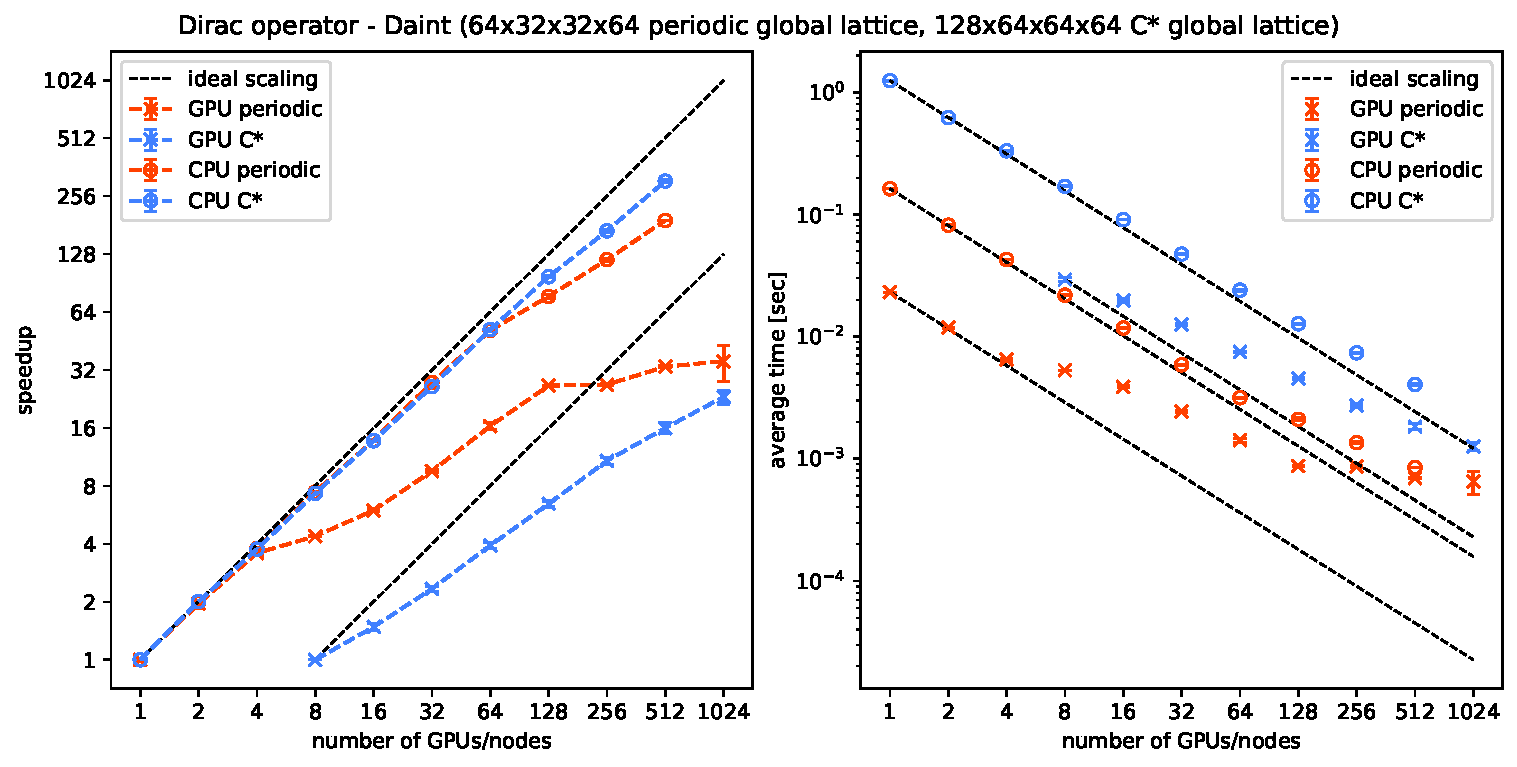
\includegraphics[width=\linewidth]{\dir/daint_dw_strong}
    \caption{Strong scaling (left) and time for one application (right) of the Dirac operator on Piz Daint (see \cref{sec:hardware}) on the CPU (circles) and GPU (crosses) using a periodic (red) and a lattice with 3 C$^\star$ directions (blue). The x-axis denotes the number of nodes for CPU runs (32 ranks per node) and number of GPUs for GPU runs (1 P100 GPU per node). The global lattice sizes are $V_\mathrm{G} = (64 \times 32 \times 32 \times 64)$ and $V_\mathrm{G} = (64 \times 64 \times 64 \times 128)$ for the periodic and C$^\star$ runs, respectively.}
    \label{fig:daint_dw_strong}
\end{figure}

\begin{figure}
    \centering
    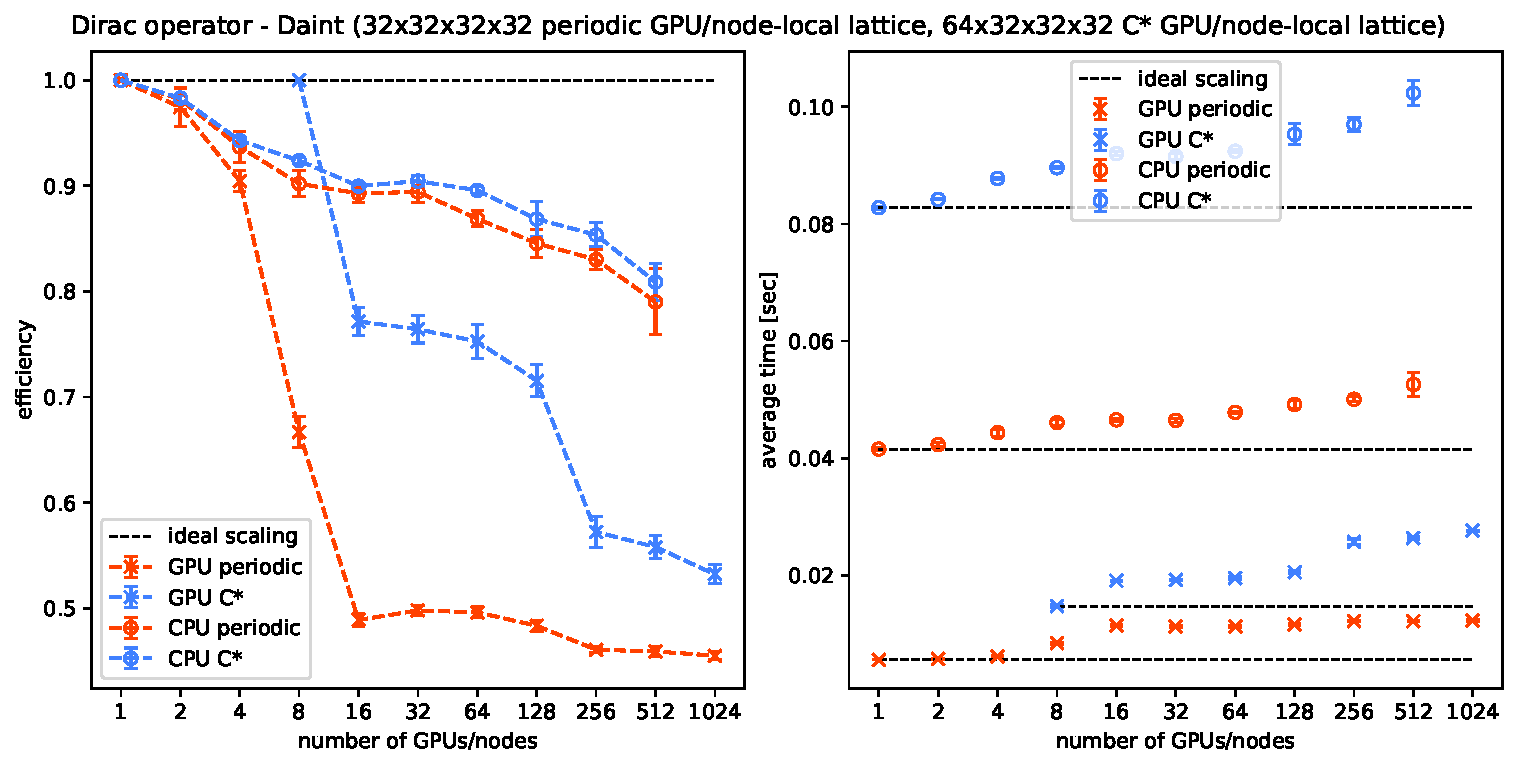
\includegraphics[width=\linewidth]{\dir/daint_dw_weak}
    \caption{Weak scaling (left) and time for one application (right) of the Dirac operator on Piz Daint (see \cref{sec:hardware}), the setup is the same as in \cref{fig:daint_dw_strong}. The node- or GPU-local lattice sizes are $V_\mathrm{L} = (32 \times 32 \times 32 \times 32)$ and $V_\mathrm{L}= (64 \times 32 \times 32 \times 32)$ for the periodic and C$^\star$ runs, respectively. Notice that the physical lattice is of the same size in both cases (the C$^\star$ lattice needs to be doubled in one of the spatial directions).}
    \label{fig:daint_dw_weak}
\end{figure}

\begin{figure}
    \centering
    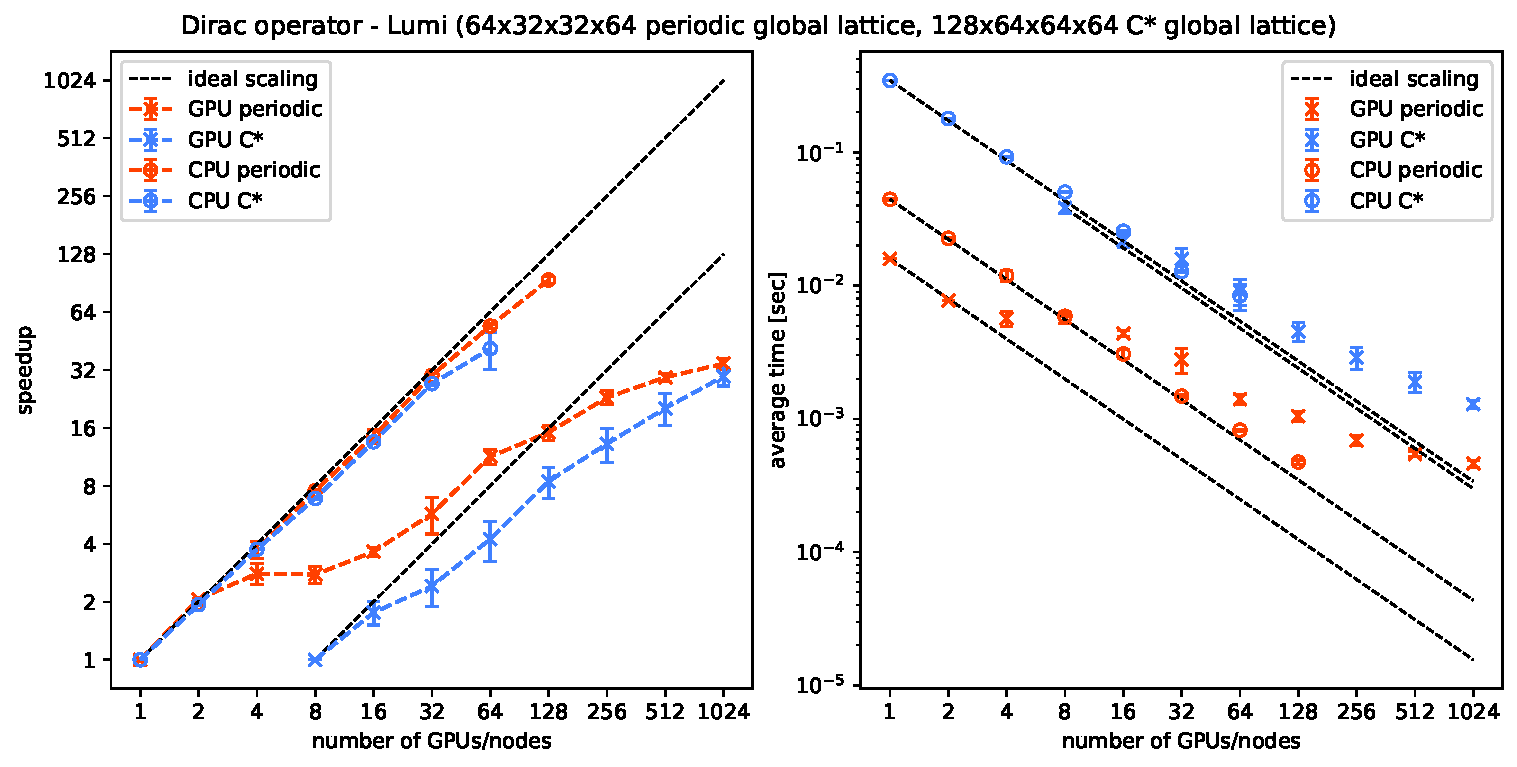
\includegraphics[width=\linewidth]{\dir/lumi_dw_strong}
    \caption{Strong scaling (left) and time for one application (right) of the Dirac operator on LUMI-G and LUMI-C (see \cref{sec:hardware}). Notice that for the x-axis, number of GPUs is not the same as the number of nodes. A LUMI-G nodes has 4x AMD MI250s, logically abstracted as 8 GPUs.}
    \label{fig:lumi_dw_strong}
\end{figure}

\begin{figure}
    \centering
    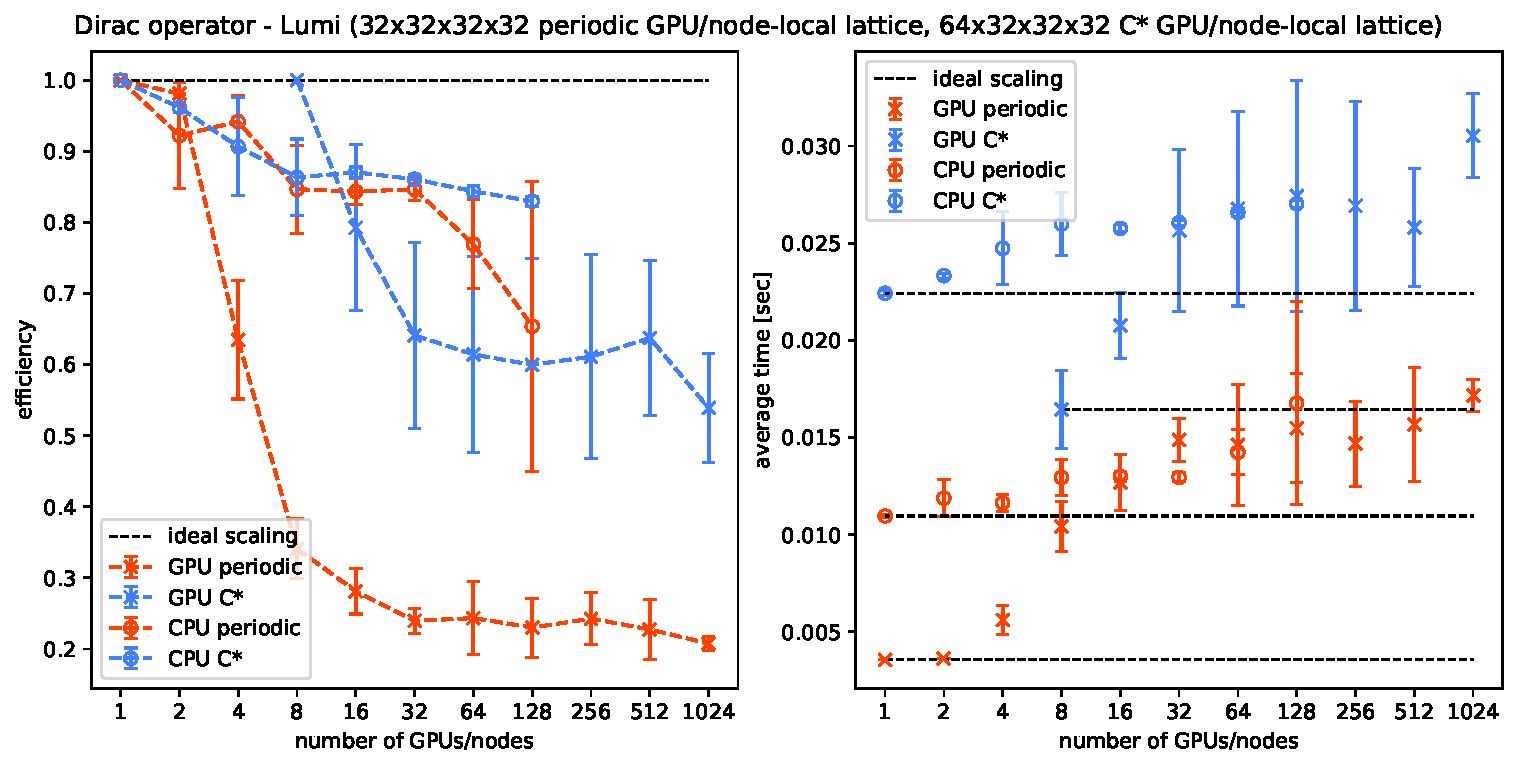
\includegraphics[width=\linewidth]{\dir/lumi_dw_weak}
    \caption{Weak scaling (left) and time for one application (right) of the Dirac operator on LUMI-G (see \cref{sec:hardware}).}
    \label{fig:lumi_dw_weak}
\end{figure}

\subsection{Solving the Dirac equation}

For solving the Dirac equation, we use a heavily preconditioned GCR algorithm. In case of the CPU runs, we use openQxD's deflated mixed-precision%
\footnote{single and double precision IEEE-754 floats} GCR solver that uses Schwarz alternating procedure as a preconditioner (\code{DFL\_SAP\_GCR} in openQCD parlance). The GPU runs use QUDAs mixed-precision%
\footnote{half, single and double precision IEEE-754 floats} multi-grid GCR solver (MG). The two solvers are very similar in how they generate the coarse grid subspace. The CPU solver parameters are tuned, but due to lack of experience with multi-grid, we used a somewhat not optimised parameter set for multi-grid on the GPU. The relative residual is chosen to be $10^{-12}$ for all solves.

We obtain good weak scaling, see \cref{fig:inv_weak}. Again, LUMI outperforms Piz Daint in terms of cost. This is expected, since one LUMI-G node contains $4$ AMD MI250s (abstracted as $8$ devices) and one Piz Daint hybrid node contains a single NVIDIA P100. The factor is not 4x, but rather $\ge10$x, which is explained by the higher memory bandwidth of the former GPU \footnote{P100: 720 GB/s \cite{online:nv_p100} vs. MI250: 3.2768 TB/s \cite{online:amd_mi250}.}.
We note that strong-scaling for multi-grid algorithms is inherently challenging due to the reduced numbers of degrees of freedom on the coarser levels, which requires new algorithmic ideas~\cite{Espinoza-Valverde:2022pci}.

% \begin{table}
% \begin{tabular}{l|l|l}
% \toprule
%  & \multicolumn{2}{c}{cost in node-seconds [sec]} \\
% \midrule
% GPUs & LUMI-G & Piz Daint \\
% \midrule
%  32 & 34.6 &  347 \\
%  64 & 70.0 &  748 \\
% 128 & 159  & 1693 \\
% 256 & 349  & 3584 \\
% 512 & 825  & 8558 \\
% \bottomrule
% \end{tabular}
% \caption{Cost in node-seconds of one solve of the Dirac equation. The GPU-local lattice is held constant ($V_\mathrm{L}=32x32x32x32$).}
% \label{tab:nodehours_inv}
% \end{table}

\begin{figure}
    \centering
    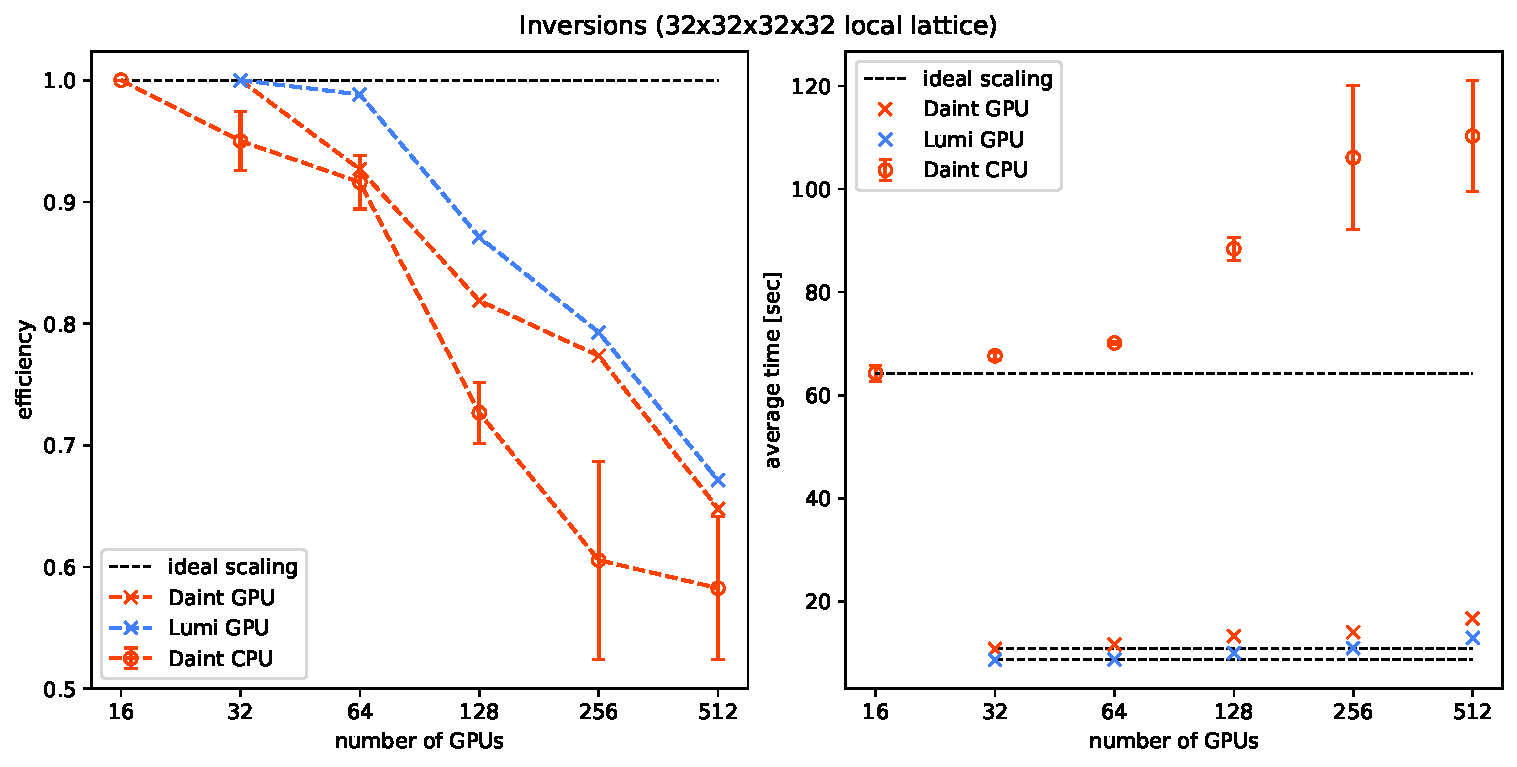
\includegraphics[width=\linewidth]{\dir/inv_weak}
    \caption{Weak scaling (left) and time to solution (right) for one solve of the Dirac equation on LUMI (blue) and on Piz Daint (red) on the CPU (circle) and GPU (crosses) partition. For specifications on the machines, see \cref{sec:hardware}.}
    \label{fig:inv_weak}
\end{figure}
